
\subsubsection{ActivityFlow}\label{sec:activityflow}
%\TODO{Link to D-PROV!}
For facilitating grouping of activities (and their related entities, etc.) we
introduce the class \class{ActivityFlow}. It can be used for hiding and grouping
a part of the workflow/pipeline  or provenance  description, if different levels
of granularity are required. Such pipelines and workflows are very common in
astronomical data production and processing. Figure
\ref{fig:provgraph-activityflow} illustrates an example provenance graph at a
detailed level (left side), and also using an \class{ActivityFlow} (right
side).


\begin{figure}[ht]
\centering
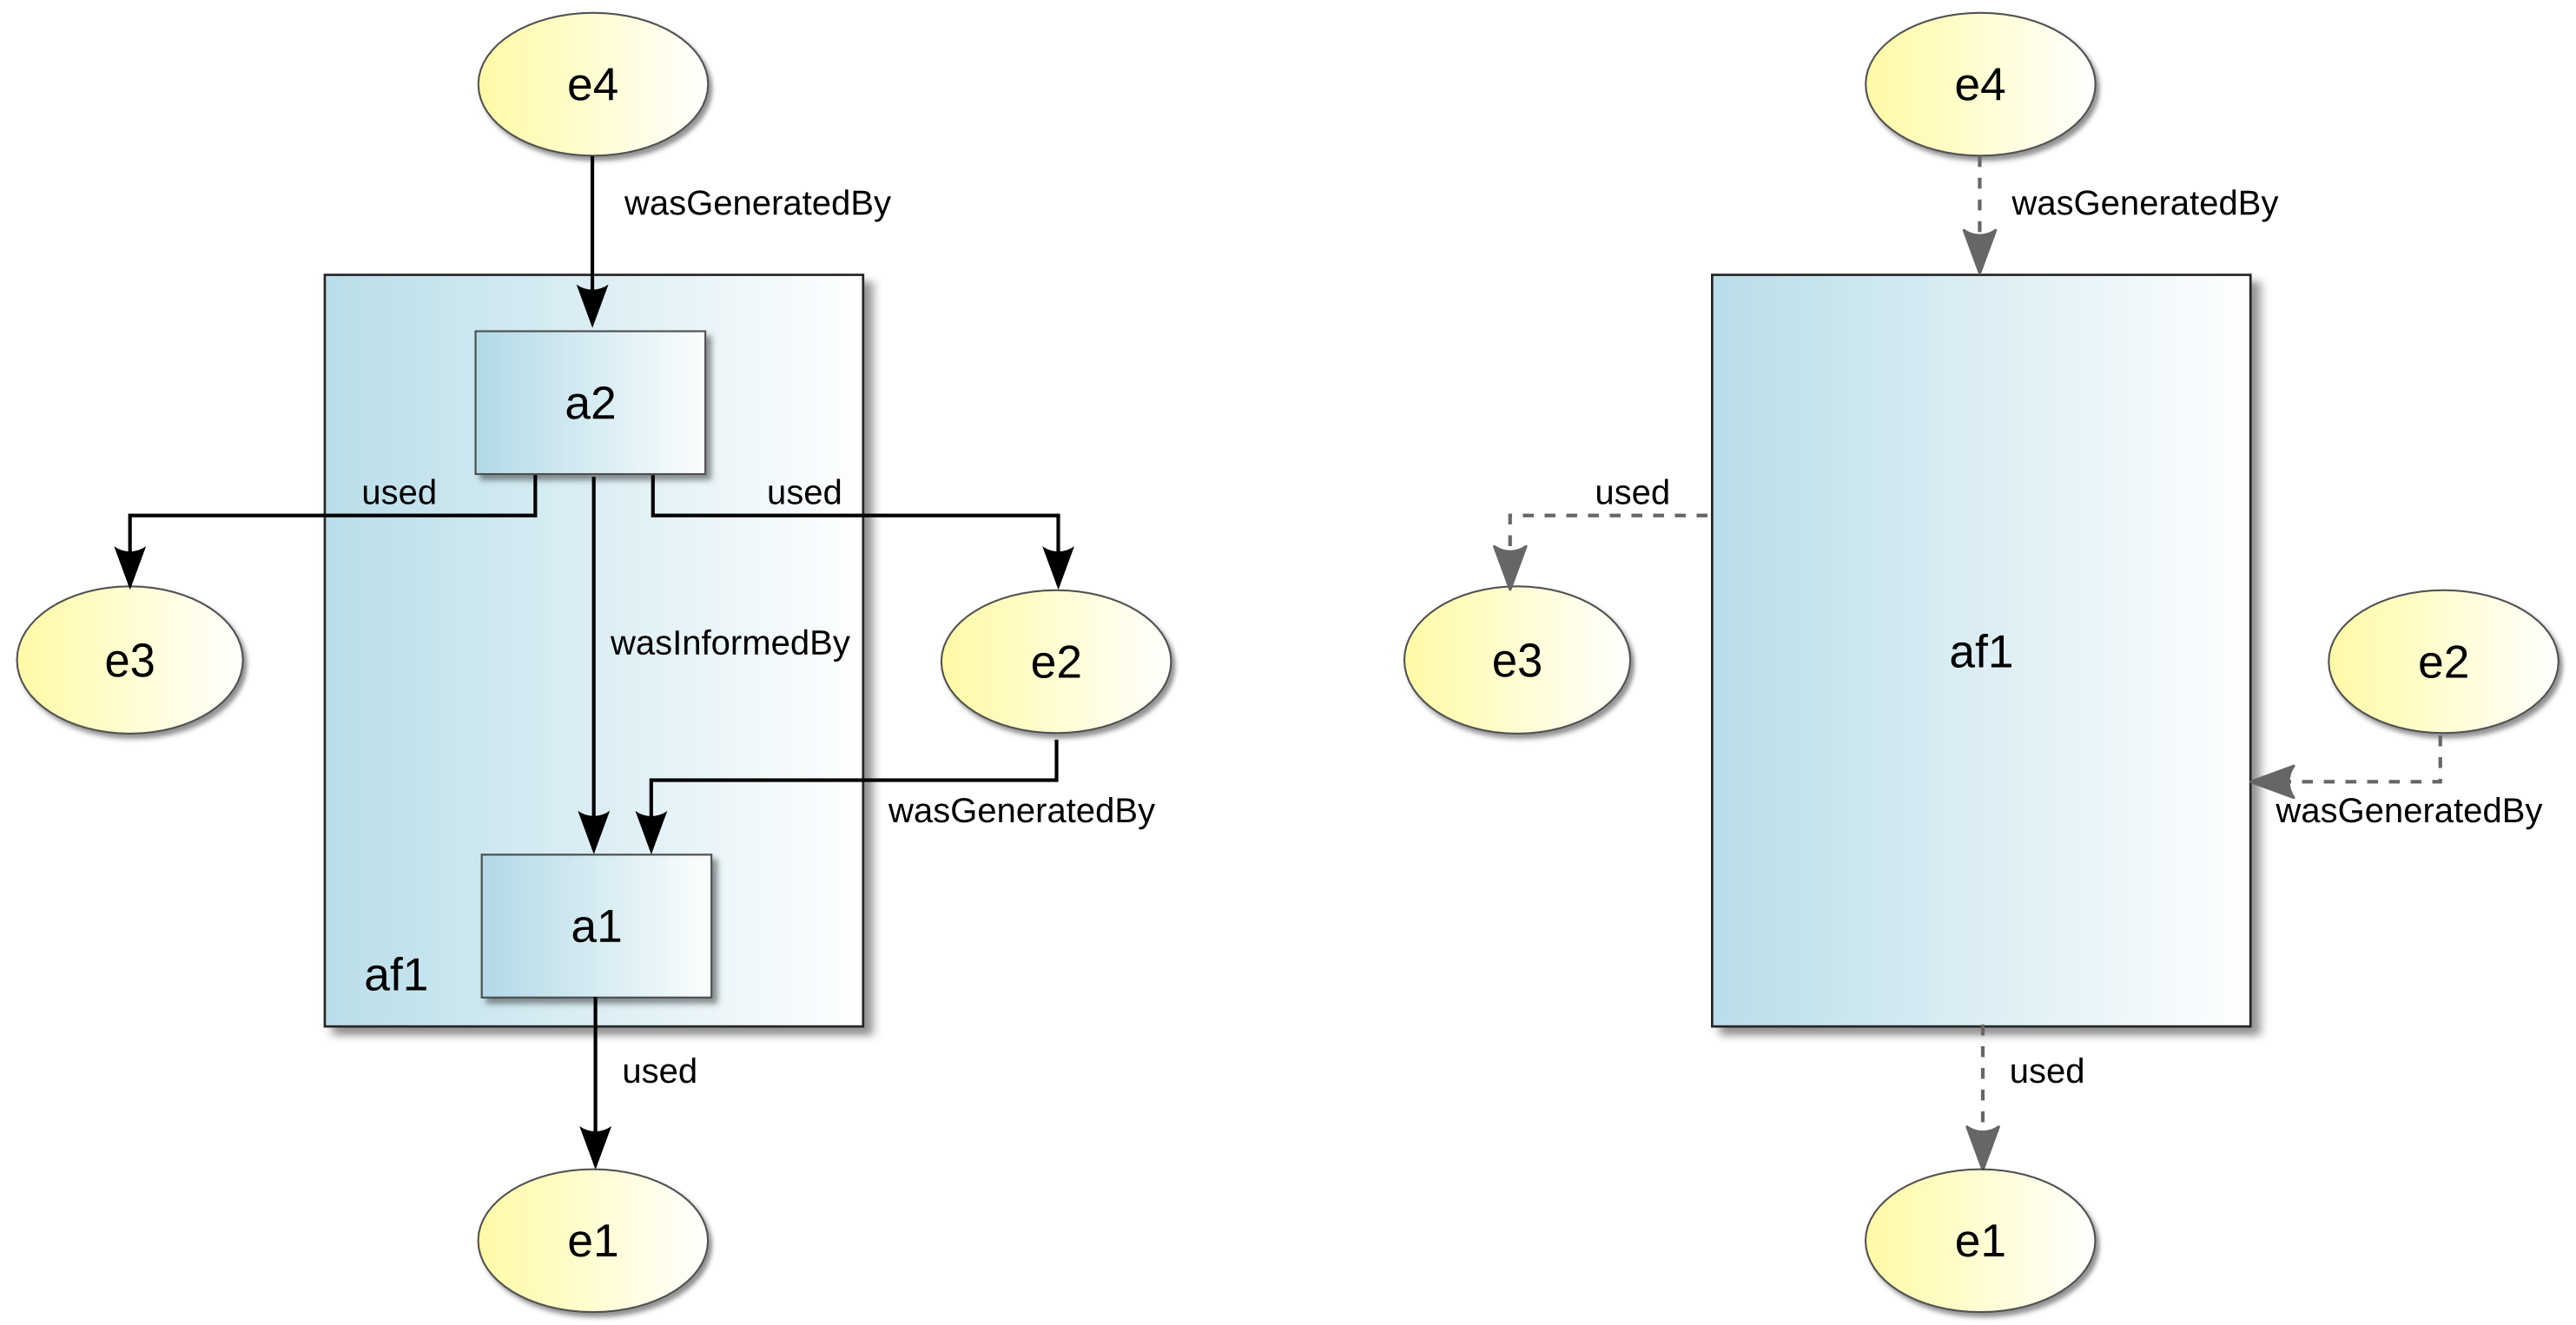
\includegraphics[width=1\textwidth]{provgraph-activityflow}
\caption[Example provenance graph with \class{ActivityFlow}]{An example provenance graph. The detailed version is shown on the left side. It also shows
the shortcut \class{WasInformedBy} to connect two activities, which could be used if the entity e2 
would not be needed anywhere else.
An ActivityFlow can be used to ``hide'' a part of the provenance graph as is shown on the right side.
Activities are marked by blue rectangles, entities by yellow ellipses.}
\label{fig:provgraph-activityflow}
\end{figure}

We also explored the different ways to describe a set of activities within the
W3C provenance model. This model uses \class{Bundle}, i.e. an entity with type
``Bundle'',  for wrapping a provenance description. Each part of a provenance
description can be  put into a bundle, and the bundle can then be reused in
other provenance descriptions.  W3C's \class{Plan} is an entity with type
``Plan'' and is used for describing a  set of actions or steps. Both,
\class{Bundle} and \class{Plan}, are entities and  have the attributes and
relations of this class (and thus one can define provenance of bundles and plans
as well).

But we would like to consider a set of activities as being an \class{Activity}
itself,  with all the relations and properties that characterize activities.
Therefore, we do not reuse W3C's classes for describing workflows and plans, but
add  the class \class{ActivityFlow} as an activity composed of other activities. The
composition is represented by  the \class{HadStep} relation, as is shown in
Figure~\ref{fig:activity-details}. In implementations, \class{ActivityFlow}
can either be represented as an extra class or as \class{Activity} with attribute \attribute{votype="ActivityFlow"}.
%while still making it obvious that this 
%group contains activities, we introduce the class \class{ActivityFlow}.
%This can be used for describing workflows or pipelines, or for 
%
%We also allow ActivityCollections to consist of a whole provenance graph of 
%activities and entities being linked together.


%We could introduce an additional abstract class, e.g. \class{AbstractActivity}, with \class{Activity} and 
%\class{ActivityFlow} being subclasses to this one. But this adds another layer of complexity 
%that we may not want in this data model.

%Since we introduced \class{ActivityFlow} mainly for having different view levels, 
%we may want to add an attribute \emph{viewLevel} to descriptions of activityflows.
% But where to set the 0 point for viewLevel???


